%\expandafter\def\csname CTEX@spaceChar\endcsname{\hspace{1em}}
\documentclass[oneside,AutoFakeBold=true]{ZJUthesisv2}
\usepackage{url}
% 该文档中首字符为“%”的均为注释行,不会在论文中出现

% 由于fontsepc包有更新,可能造成在编译过程中的问题
% 如果使用ZJUthesis有问题,可尝试使用ZJUthesisv2
% 如果仍有问题,可换回ZJUthesis,尝试将下面的一行拷至本文档\documentclass之前
% \expandafter\def\csname CTEX@spaceChar\endcsname{\hspace{1em}}

% 论文默认为单面模式,需双面模式请将第一行换为如下所示:
% \documentclass[twoside]{ZJUthesis}
% AutoFakeBold=true 是为解决在Windows系统下,使用xelatex时中文字体不能加粗的问题

% 取消目录中链接的颜色,方便打印
% 如需颜色,请将“false”改为“true”
\hypersetup{colorlinks=false}

%\usepackage[sectionbib]{chapterbib}

\begin{document}
%%%%%%%%%%%%%%%%%%%%%%%%%%%%%
%% 正文字体设定
%%%%%%%%%%%%%%%%%%%%%%%%%%%%%
\fangsong

%%%%%%%%%%%%%%%%%%%%%%%%%%%%%
%% 论文封面部分
%%%%%%%%%%%%%%%%%%%%%%%%%%%%%
% 中文封面内容

% 中图分类号
\classification{TP391.7}

% 单位代码
\serialnumber{10335}

% 密级,如需密级则将其前“%”去掉
%\SecretLevel{绝密}

% 学号
\PersonalID{11521033}

\title{基于深度视频的物体形变捕捉}
% 如果标题一行写不下,就写成两行,在下面的命令里写第二行,不需要两行则注释掉
\titletl{和子空间构建}
%\titletl{test}

%英文题目
\Etitle{Deformation Capture and Subspace}
% 如果一行写不下,同中文题目设定,一行写不下则写两行,不需要就注释掉
\Etitletl{Building with Depth Video}

% 作者
\author{王\hspace{1.5em}子\hspace{1.5em}豪}

\degree{硕士}

% 导师
\supervisor{侯启明\hspace{1em} 副教授}
%\supervisor{郑友怡\hspace{1em} 研究员}

% 合作导师,如果有的话,去掉注释,
\cpsupervisor{郑友怡\hspace{1em} 研究员}

% 专业名称
\major{计算机科学与技术}

% 研究方向
\researchdm{计算机图形学}

% 所属学院
\institute{计算机科学与技术学院}

%论文提交日期
\submitdate{2018年3月20日}

% 答辨日期
\defenddate{2018年9月20日}

% 生成封面
\makeCoverPage


%%%%%%%%%%%%%%%%%%%%%%%%%%%%%%
%% 中文题名页内容
%%%%%%%%%%%%%%%%%%%%%%%%%%%%%%
% 论文评阅人信息 注意两字名与三字名,两字职称与三字职称的写法,便于对齐
% 多余的名额直接注释掉即可,比如三个评阅人,把评阅人D,E注释掉即可
\reviewersA{丘处机\hspace{1.5em}真人\hspace{1.5em}登州滨都宫\hspace{1em}}
\reviewersB{葛\quad 洪\hspace{1.5em}方士\hspace{1.5em}罗浮山道观\hspace{1em}}
\reviewersC{寇谦之\hspace{1.5em}天师\hspace{1.5em}嵩山中岳道场}
\reviewersD{张三丰\hspace{1.5em}真君\hspace{1.5em}武当玉虚宫\hspace{1em}}
\reviewersE{孙玄清\hspace{1.5em}真人\hspace{1.5em}崂山明霞洞\hspace{1em}}

% 答辩委员会信息,如果某一个单位比较长,
% 请在其它较短后面补上{hspace{Xem}},X是比最长的单位名少几个字
% 如果实际人数少于6人,多余的注释掉即可
\chairman{唐三藏\hspace{1.5em}功佛\hspace{1.5em}洛阳大慈恩寺}
\commissionerA{惠\quad 能\hspace{1.5em}方丈\hspace{1.5em}曹溪宝林寺\hspace{1em}}
\commissionerB{智\quad 顗\hspace{1.5em}方丈\hspace{1.5em}天台山国清寺}
\commissionerC{法\quad 藏\quad 大和尚\quad 洛阳佛授记寺}
\commissionerD{道\quad 济\hspace{1.5em}和尚\hspace{1.5em}临安灵隐寺\hspace{1em}}
\commissionerE{降\quad 龙\hspace{1.5em}尊者\hspace{1.5em}天竺大雷音寺}

% 生成中文题名页
\maketitle


%%%%%%%%%%%%%%%%%%%%%%%%%%%%%%
%% 英文封面内容,硕士论文可不要此页
%%%%%%%%%%%%%%%%%%%%%%%%%%%%%%
% 英文题名
\englishtitle{HVlab~\LaTeX~Fast Guide}
% 如果题名一行写不下,就写到第二行,不需要则将其注释掉
\englishtitletl{The Second Edition}

% 评阅人信息,名字,职称,单位尽量用简写,否则会写不下
\EreviewersA{Name\hspace{1.5em}Professional Title\hspace{1.5em}Organization}
\EreviewersB{Name\hspace{1.5em}Professional Title\hspace{1.5em}Organization}
\EreviewersC{Name\hspace{1.5em}Professional Title\hspace{1.5em}Organization}
\EreviewersD{Name\hspace{1.5em}Professional Title\hspace{1.5em}Organization}
\EreviewersE{Name\hspace{1.5em}Professional Title\hspace{1.5em}Organization}

% 答辩委员会信息,同样尽量用简写,否则会写不下
\Echairman{Name\hspace{1.5em}Professional Title\hspace{1.5em}Organization}
\EcommissionerA{Name\hspace{1.5em}Professional Title\hspace{1.5em}Organization}
\EcommissionerB{Name\hspace{1.5em}Professional Title\hspace{1.5em}Organization}
\EcommissionerC{Name\hspace{1.5em}Professional Title\hspace{1.5em}Organization}
\EcommissionerD{Name\hspace{1.5em}Professional Title\hspace{1.5em}Organization}
\EcommissionerE{Name\hspace{1.5em}Professional Title\hspace{1.5em}Organization}

% 生成英文封面
%\makeenglishtitle


%%%%%%%%%%%%%%%%%%%%%%%%%%%%%%
%% 原创声明与版权协议页
%%%%%%%%%%%%%%%%%%%%%%%%%%%%%%

\SignautreDateA{2018}{9}{11}
\SignautreDateB{2018}{9}{11}
\SignautreDateC{2018}{9}{11}
% 生成原创声明与版权协议页
\makeOSandCPRTpage


%%%%%%%%%%%%%%%%%%%%%%%%%%%%%%
%% 论文部分开始
%%%%%%%%%%%%%%%%%%%%%%%%%%%%%%
\ZJUfrontmatter

%%%%%%%%%%%%%%%%%%%%%%%%%%%%%%
%% 勘误页,一般没有
%%%%%%%%%%%%%%%%%%%%%%%%%%%%%%
%\expandafter\def\csname CTEX@spaceChar\endcsname{\hspace{1em}}
\begin{corrigenda}
这是一个勘误\index{勘误}章节,一般情况下是没有的。
\end{corrigenda}


%%%%%%%%%%%%%%%%%%%%%%%%%%%%%%
%% 致谢页
%%%%%%%%%%%%%%%%%%%%%%%%%%%%%%
%\begin{thanks}
% 光阴似箭,我在浙江大学的求学生涯以及接近尾声。
% 在这几年中,我经历了很多,学习了很多,收获了很多,也成长了很多。

% 首先我要感谢我的父母和其他关心我的家人,
% 使他们无怨无悔的付出和全心全意的支持让我没有后顾之忧,
% 能够专心学业与科研。

% 衷心感谢我的导师侯启明副教授、周昆教师和郑友怡老师对我的悉心指导。
% 他们不仅授予我丰富的知识,
% 还培养了我良好的工作科研的习惯与态度。
% 他们在科研上严格的要求,严谨的治学态度和深厚的学术造诣一直在我求学的道路上指引着我。

% 由衷感谢实验室的所有同学们。
% 是他们的陪伴让我的研究生生活充满斑斓的色彩;
% 是他们的帮助帮我解决了学习中科研中遇到的众多问题。

% 最后我要感谢所有评阅论文和答辩委员会的各位老师,
% 感谢你们在百忙之中给予我指导。
由于论文送审需要,隐去本章节。
\end{thanks}


%%%%%%%%%%%%%%%%%%%%%%%%%%%%%%
%% 序言页
%%%%%%%%%%%%%%%%%%%%%%%%%%%%%%
%\include{./Chapters/preface}

%%%%%%%%%%%%%%%%%%%%%%%%%%%%%%
%% 摘要
%%%%%%%%%%%%%%%%%%%%%%%%%%%%%%
\begin{abstract}
与三维模型形变有关的相关技术一直许多研究关注的问题,
在动画制作和游戏开发等领域也有着广泛的应用。
而随着近年来消费级深度相机的的普及,
使得基于深度相机研究与应用越来越多。

本文提出了一种基于RGBD视频的形变子空间技术。
本文以RGBD相机采集的RGBD视频为输入,
实现了从三维模型重建、物体位姿估计、形变捕捉、形变子空间构建的流程。
基于形变子空间的模型修改方法能够保证修改的模型符合物体本身的形变特征。
本文的工作可主要分为四步:
首先,本文会用深度相机扫描物体,
捕捉物体表面的形状信息,
并据此重建三维模型。
然后本文会以RGBD图像为输入,
根据操作者的手部信息分割出属于深度图像中属于物体的部分,
并据此估计出物体的初始位姿。
这一步可看做形变捕捉的预处理。
然后本文会以深度视频为输入,
用基于双四元数的形变图描述模型的形变,
通过优化形变图参数捕捉物体的形变,
并挑选出有代表性的形变状态作为形变关键帧。
最后本文会从形变关键帧中提取出基于形变梯度的特征向量,
以这些特征向量作为基向量张成非线性的特征空间。
特征空间中的特征向量对应的形变模型构成了模型的形变子空间。
此外本文还给出了基于形变子空间的模型形状修改方法,
保证修改的模型尽可能落在形变子空间内。

由于本文的三维模型和形变关键帧都是借助RGBD相机捕捉物体的表面信息获得,
并不是通过手工的编辑获得,
所以能保证静态的三维模型和形变关键帧都是符合物体本身的特点的。
所以由此构建出的形变子空间是较为合理的。

\keywords{RGBD相机 ,双四元数,形变捕捉,形变子空间}
\end{abstract}


%%%%%%%%%%%%%%%%%%%%%%%%%%%%%%
%% 英文摘要
%%%%%%%%%%%%%%%%%%%%%%%%%%%%%%
\begin{englishabstract}


\TeX\index{\TeX}

\englishkeywords{\TeX}

\end{englishabstract}


%%%%%%%%%%%%%%%%%%%%%%%%%%%%%%
%% 插图列表
%%%%%%%%%%%%%%%%%%%%%%%%%%%%%%
\ZJUListofFigures

%%%%%%%%%%%%%%%%%%%%%%%%%%%%%%
%% 表格列表
%%%%%%%%%%%%%%%%%%%%%%%%%%%%%%
\ZJUListofTables

%%%%%%%%%%%%%%%%%%%%%%%%%%%%%%
%% 缩写、符号清单、术语表
%%%%%%%%%%%%%%%%%%%%%%%%%%%%%%
%\include{./Chapters/symbol}

%%%%%%%%%%%%%%%%%%%%%%%%%%%%%%
%% 目录页
%%%%%%%%%%%%%%%%%%%%%%%%%%%%%%
\ZJUcontents


%%%%%%%%%%%%%%%%%%%%%%%%%%%%%%
%% 正文内容部分开始
%%%%%%%%%%%%%%%%%%%%%%%%%%%%%%
\ZJUmainmatter


\chapter{绪论}

%1.1课题背景

\section{课题背景}
三维模型的获取和编辑方面的研究有着悠久的历史,在工业界也有着十分广泛的应用。
随着近年来游戏、动画产业的高速发展,工业界对于三维模型的需求量也日益增加。
因此,如何高效的获取三维模型,如何有效的编辑三维模型的姿态逐渐成为学术界和工业界共同关注的问题。

三维模型的构建过程通常称为三维建模。对于现实世界中已经存在的物体,业内通常通过三维扫描的方式建模。
搭载深度摄像头的三维扫描设备不仅能获取视野中的颜色信息,还能通过三维测距技术获取深度信息。
传统的三维扫描设备价格昂贵、操作复杂,通常在较为专业的领域使用。
近年来,消费级深度相机越来越普及,Microsoft、Google、Apple等科技巨头也纷纷推出了搭载了深度相机的产品。
这使得通过三维扫描获得三维模型越来越容易,基于深度的信息的相机的应用场景也越来越多。

在游戏、动画等领域,仅仅用一个静态的三维模型描述一个物体是远远不够的,它们需要以许多不同的姿态、形状出现。
显然,通过修改原有模型生产新的三维模型可以大幅降低建模成本。
使三维模型改变姿态、形状,需要修改其三维信息。以多边形网格模型为例,需要修改顶点的三维坐标。
直接修改网格模型的每个顶点的位置显然不现实,
现有的模型修改工具通常通过修改少数控制点使模型在符合一定约束的情况下发生形变,从而得到新的模型。
在修改模型的过程中,可能会使模型产生不符合物体特性的形变。
如何方便的修改模型,如何保证模型在修改的过程中发生的形变尽量合理一直是业内关注的问题。


\section{本文工作}
本文借助了深度相机,以RGBD视频作为输入,
完成了一个从三维模型重建、位姿估计、模型形变捕捉到模型形变子空间构建的流程。
深度视频由按照时间顺序排列的深度图像构成。
与普通的图像不同,深度图像将场景中采样点距图像采集器的距离,即深度,作为其像素值,
它能够直观的描述场景的几何信息。
基于深度图像中记录的几何信息,本文实现了物体的三角网格模型的重建以及模型形变的捕捉,
并基于捕捉到的形变信息,构建了模型的合理的形变子空间,
使得模型在被修改的过程中发生的形变尽可能的接近落在这个子空间内的形状。

本文利用深度相机扫描物体,基于扫描过程中采集的深度信息重建三维模型。
深度图像记录了物体表面上的采样点与相机的相对位置。在扫描的过程中,本文会跟踪相机的运动轨迹,
得到每一帧的相机位置,从而计算出物体在全局坐标系中的位置。
在重建的步骤中,本文用体素描述三维模型,并根据每一帧深度图像更新体素的值。
体素模型可通过Matching Cubes\cite{lorensen1987marching}算法转换为三角网格模型。

在形变捕捉之前,本文需要估计物体的初始位姿。
本文首先从由RGBD图片生成的点云中分割出手部点云,
再通过手部点云的位置分割出物体的点云。
最后通过让网格模型与物体点云对齐估计出物体的初始位姿作为形变捕捉的初始位姿。

在获得了物体的静态三维模型和初始位姿后,本文需要用户摆弄物体使之发生形变,
并利用深度相机捕捉物体的形变,得到模型的形变关键帧。
在形变捕捉阶段,本文以静态三维模型与记录了物体形变过程的深度视频作为算法的输入,
得到一组形变后的模型作为该模型的形变关键帧。
本文用基于双四元数的形变图描述模型的形变。
对于每一帧,本文会优化形变图的参数,令形变后的模型和深度图像尽可能吻合,
从而得到发生形变后的模型,并挑选其中具有代表性的形变模型作为模型的形变关键帧。

然后,本文会从形变关键帧中提取出特征向量,构建模型的形变子空间。
从形变关键帧中提取的的特征向量描述了形变模型相对于静态模型的相对形变。
当静态模型已知时,特征向量和形变模型可以互相转换。
从形变关键帧中提取的特征向量称为关键向量,由特征向量张成的空间称为特征空间,即模型的形变子空间。
用户可以通过修改少数控制点修改模型,求解出一个落在特征空间内的特征向量和各个顶点的位置,
使得求解得到的模型形状和特征向量对应的形状尽可能接近。
由于形变关键帧是通过捕捉现实中物体的形变得到,所以所有的形变关键帧都是合理的,
由关键向量张成的形变子空间也是较为合理的。

算法\ref{alg_main_alg}是算法整体流程的伪代码。
其中第1行至第6行为三维重建的流程,将在第三章详细描述;
第7行至第10行为初始位姿估计流程,将在第四章详细描述;
第11行至第16行为形变捕捉与形变关键帧提取的流程,将在第五章详细描述;
第17至第20行为形变子空间构建的流程,将在第六章详细描述。
\begin{algorithm}
    %\fangsong
    \caption{本文算法流程}
    \label{alg_main_alg}
    \begin{algorithmic}[1]
        \For{each time $t$}
            \State Get depth frame
            \State Estimate the camera pose
            \State Fuse depth data into the global volume
        \EndFor
        \State Fetch mesh from the global volume
        \State Get RGBD frame for initial pose estimating
        \State Segment the hand point cloud
        \State Segment the object point cloud
        \State Match the mesh to the object point cloud to get the  initial pose
        \For{each time $t$}
            \State Get depth frame
            \State Optimize deformation parameters
        \EndFor
        \State Select representative deformation keyframes
        \State Align keyframes to the initial mesh
        \For{each keyframes}
            \State Fetch feature vector from keyframe
        \EndFor
        \State Build subspace with feature vectors
    \end{algorithmic}
\end{algorithm} 

\section{篇章结构}
本文章节安排如下:

第一章介绍了本文的研究背景以及所做的工作。

第二章回顾了研究现状与相关工作。





\chapter{研究现状与相关工作}

\chapter{基于深度相机的静态模型的采集与预处理}
 本文通过捕捉物体形变获取形变关键帧,然后根据关键帧相对于静态模型的相对形变构建形变子空间,
 这些工作都需要获取物体的静态模型作为参照。
 本章的目的就是获取一个物体静态三维模型,作为后续形变捕捉与形变子空间构建的输入。
\begin{figure}[h]
    \centering
    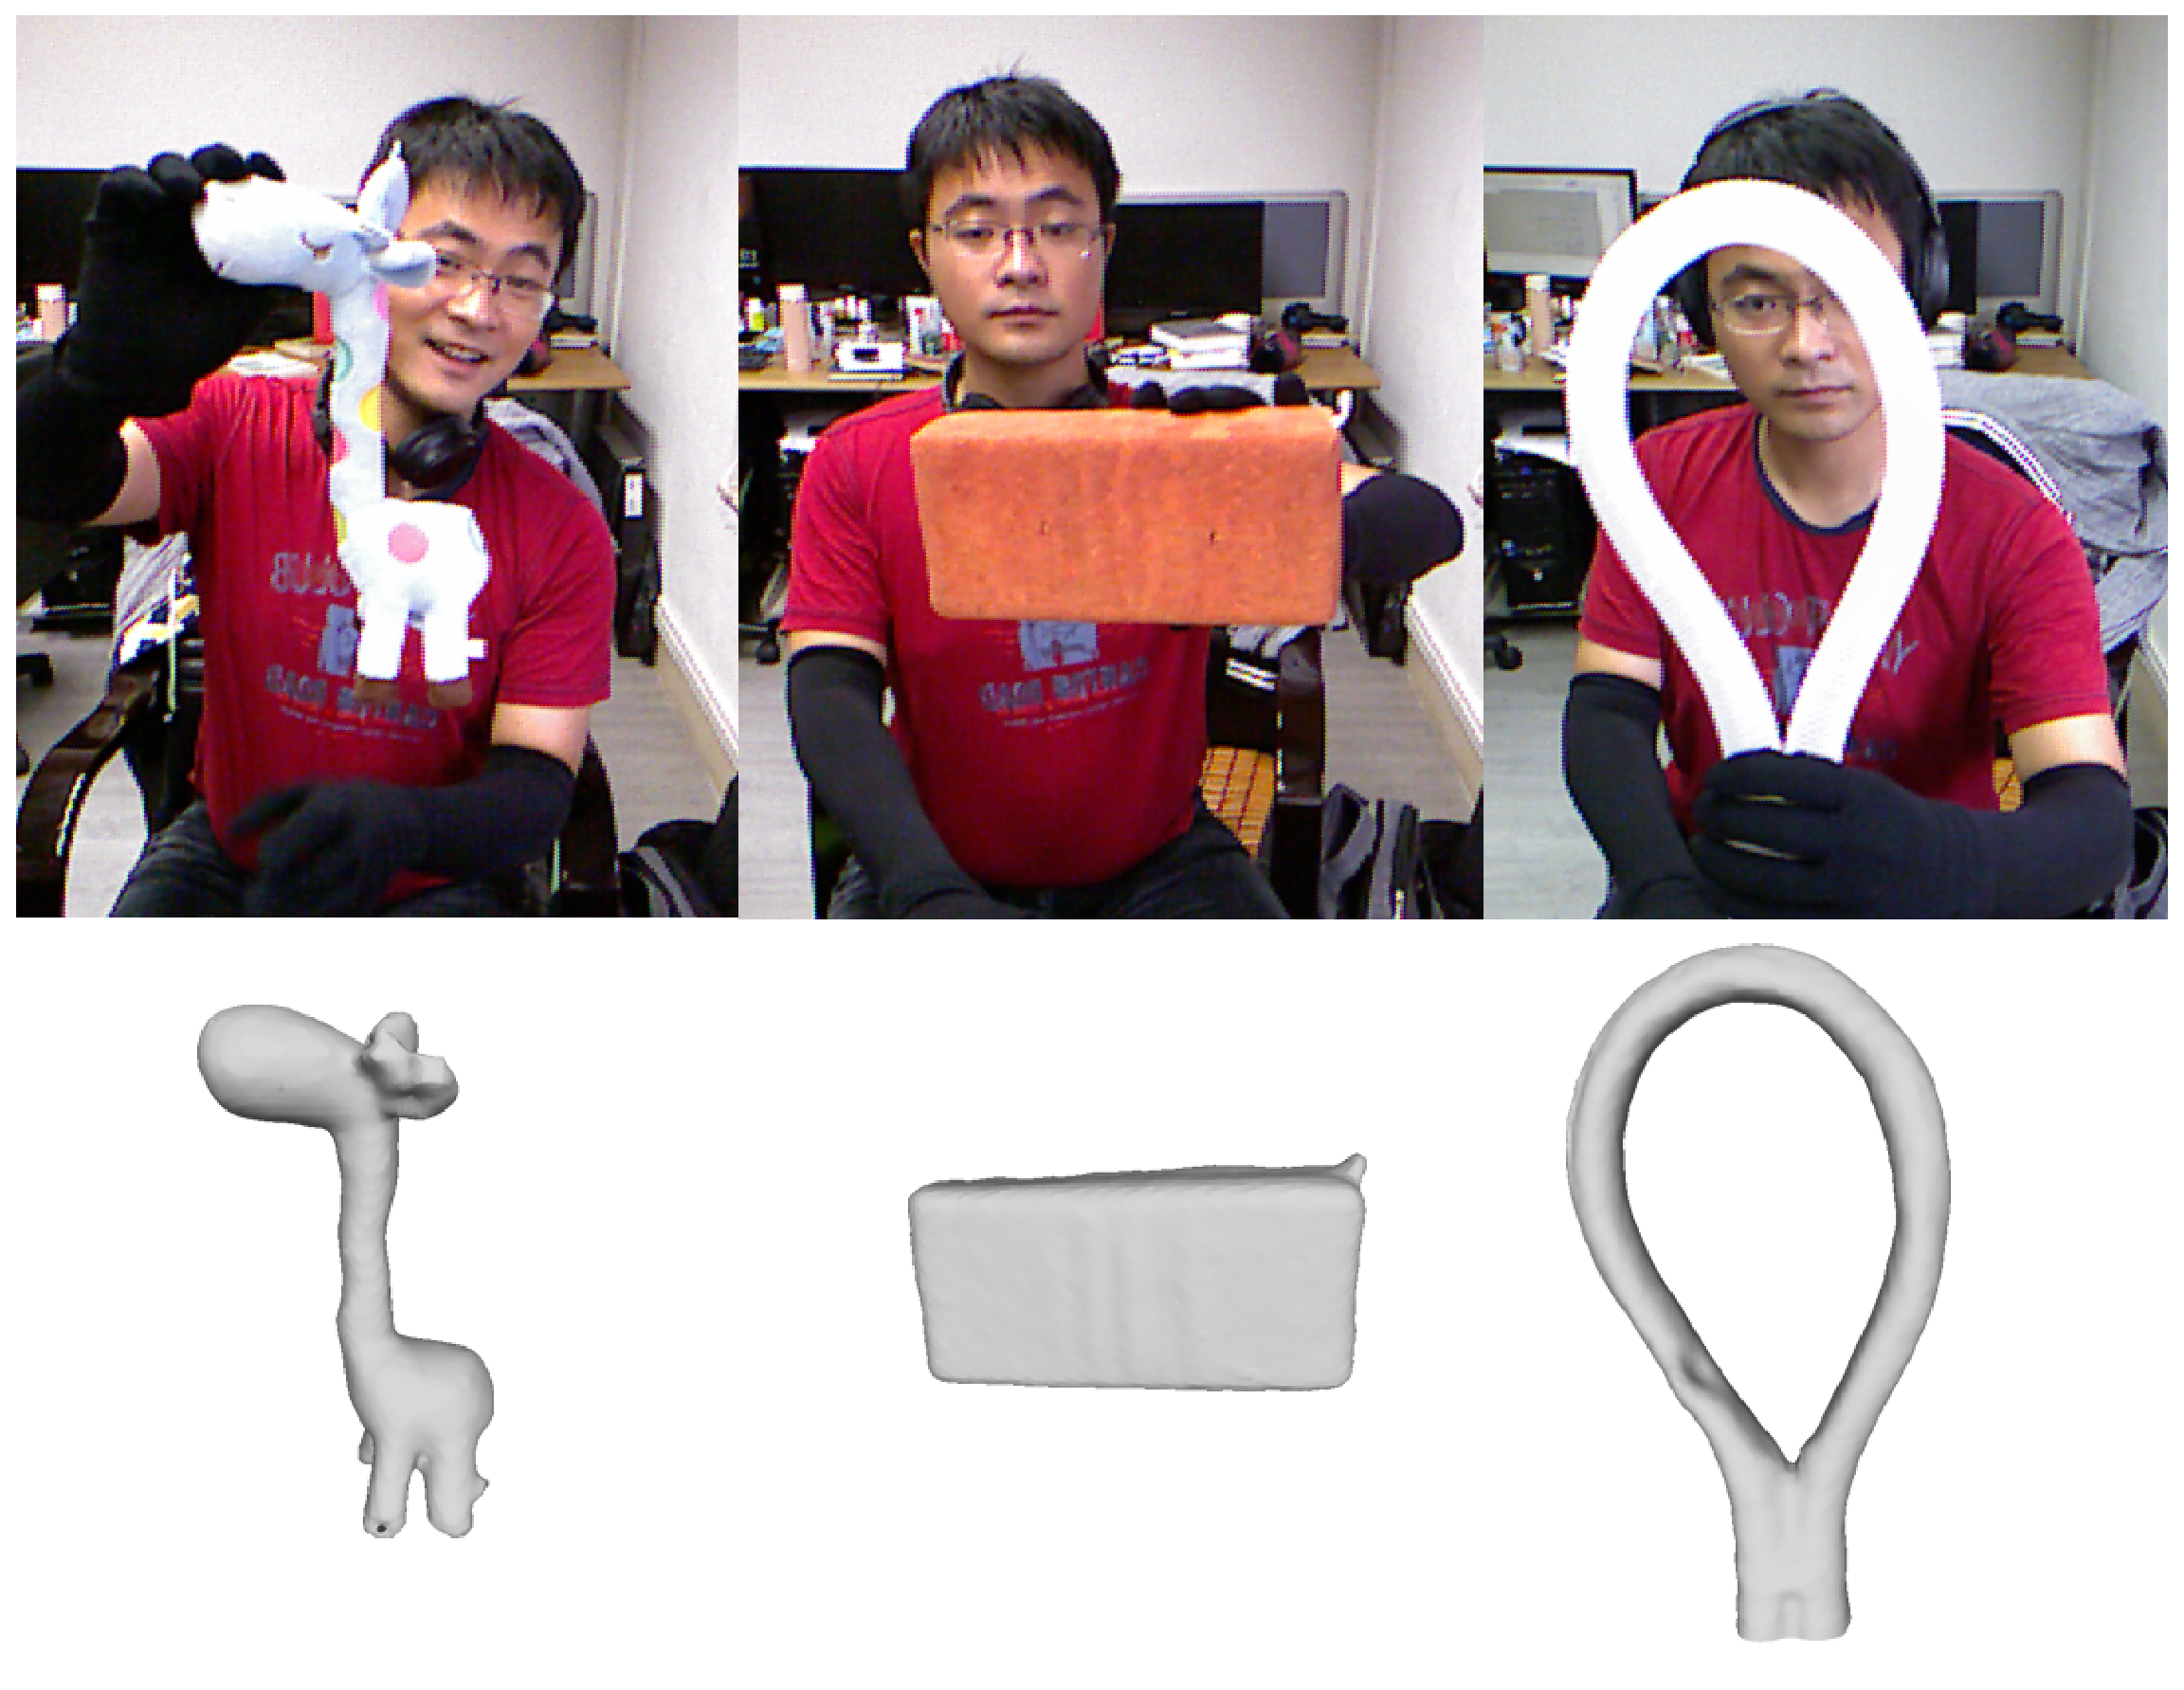
\includegraphics[width=0.9\textwidth]{./Pictures/static_mesh.eps}
    \caption{采集静态模型}
    \label{static_model}
\end{figure}

\section{基于深度相机的三维重建}
对于现实世界中存在的物体,其三维模型通常可以通过CAD软件建模或者借助扫描设备重建。
本文所使用的模型均借助深度相机重建。

深度相机是一种可以获取深度信息的设备,即能够测量物体表面距离相机的距离。
如同章节\ref{range_finding}所说,现在较为流行的三维测距技术有飞行时间、三角测距和结构光。
本文采用的是Microsoft生成的Kinect一代,这是一台基于结构光技术的深度相机。
Kinect除了能够获得RGB图像外,还能获得深度图像。
深度图像的每个像素记录的是物体表面距离相机的距离,
利用透视原理,可以推算出物体表面和相机的相对位置。
三维重建算法就可以通过扫描过程中获取的深度信息重建出物体的几何信息,获得三维模型。
本文采用的是KinectFusion算法\cite{izadi2011kinectfusion},
能够实时的借助深度相机重建三维模型。
KinectFusion算法\cite{izadi2011kinectfusion}以深度视频(由深度图像组成的图像流)为输入。
对于每一帧,会计算物体和相机的相对位置(物体在相机坐标系中的位置)
以及相机在世界坐标系(通常是第一帧的相机坐标)中的位置,
并将每一帧获得的数据融合到一个统一的模型坐标系中,从而得到三维模型。






\ZJUbackmatter
%%%%%%%%%%%%%%%%%%%%%%%%%%%%%%
%% 参考文献
%%%%%%%%%%%%%%%%%%%%%%%%%%%%%%
\ZJUthesisbib{mybib}

%%%%%%%%%%%%%%%%%%%%%%%%%%%%%%
%% 附录
%%%%%%%%%%%%%%%%%%%%%%%%%%%%%%
%\appendix
%\chapter{附录A}

这是附录A的内容。

\chapter{附录B}

这是附录B的内容。


%%%%%%%%%%%%%%%%%%%%%%%%%%%%%%
%% 索引
%%%%%%%%%%%%%%%%%%%%%%%%%%%%%%
%\ZJUindex

%%%%%%%%%%%%%%%%%%%%%%%%%%%%%%
%% 个人简历
%%%%%%%%%%%%%%%%%%%%%%%%%%%%%%
\begin{resume}
\begin{enumerate}
\item{第一条的内容}
\item{第二条内容}
\end{enumerate}
\end{resume}


%%%%%%%%%%%%%%%%%%%%%%%%%%%%%%
%% 发表论文目录
%%%%%%%%%%%%%%%%%%%%%%%%%%%%%%
%\begin{publications}
\begin{enumerate}
\item{第一篇}
\item{第二篇}
\end{enumerate}
\end{publications}


\end{document}
